 \let\negmedspace\undefined
\let\negthickspace\undefined
\documentclass[journal]{IEEEtran}
\usepackage[a5paper, margin=10mm, onecolumn]{geometry}
\usepackage{lmodern} % Ensure lmodern is loaded for pdflatex
\usepackage{tfrupee} % Include tfrupee package

\setlength{\headheight}{1cm} % Set the height of the header box
\setlength{\headsep}{0mm}     % Set the distance between the header box and the top of the text

\usepackage{gvv-book}
\usepackage{gvv}
\usepackage{cite}
\usepackage{amsmath,amssymb,amsfonts,amsthm}
\usepackage{algorithmic}
\usepackage{graphicx}
\usepackage{textcomp}
\usepackage{xcolor}
\usepackage{txfonts}
\usepackage{listings}
\usepackage{enumitem}
\usepackage{mathtools}
\usepackage{gensymb}
\usepackage{comment}
\usepackage[breaklinks=true]{hyperref}
\usepackage{tkz-euclide} 
\usepackage{listings}
\usepackage{gvv}                                        
\def\inputGnumericTable{}                       
\usepackage[latin1]{inputenc}                                
\usepackage{color}                                            
\usepackage{array}                                            
\usepackage{longtable}                                       
\usepackage{calc}                                             
\usepackage{multirow}                                         
\usepackage{hhline}                                           
\usepackage{ifthen}                                           
\usepackage{lscape}  
\usetikzlibrary{patterns}
\begin{document}
\bibliographystyle{IEEEtran}


\textbf{Question 3.3.10:} \\
\textbf{}  Construct a right triangle $ABC$ with $AB = 6 \, \text{cm}$, 
$BC = 8 \, \text{cm}$ and $\angle B = 90^\circ$. Draw $BD$, the perpendicular 
from $B$ on $AC$. Draw the circle through $B, C$ and $D$ and construct the 
tangents from $A$ to this circle. 


\textbf{Solution:}\\
 \textbf{Given} 
 
Let us place the triangle in coordinate geometry using vectors.

Let:
\begin{align}
\vec{b} = \myvec{0 \\ 0}, \quad \vec{a} = \myvec{6 \\ 0}, \quad \vec{c} = \myvec{0 \\ 8} \label{1}
\end{align}

Since \(\angle B = 90^\circ\), triangle \(ABC\) is right-angled at \(B\).

---

\subsection*{Finding point \( \vec{d} \): foot of perpendicular from \( \vec{b} \) to \( \vec{a} - \vec{c} \)}

Let \(\vec{n} = \vec{a} - \vec{c} = \myvec{6 \\ 0} - \myvec{0 \\ 8} = \myvec{6 \\ -8}\) \label{2}

Let the general point on line \(AC\) be:
\begin{align}
\vec{r} = \vec{c} + \lambda(\vec{a} - \vec{c}) = \vec{c} + \lambda \vec{n} \label{3}
\end{align}

The foot of the perpendicular from \( \vec{b} \) to line \( \vec{r} \) is the point on \(AC\) closest to \(\vec{b}\).

Minimize the square of the distance:
\begin{align}
\| \vec{r} - \vec{b} \|^2 = (\vec{c} + \lambda \vec{n} - \vec{b})^\top (\vec{c} + \lambda \vec{n} - \vec{b}) \label{4}
\end{align}

Differentiate w.r.t. \(\lambda\) and set derivative to zero:
\begin{align}
\frac{d}{d\lambda} \left[ \| \vec{r} - \vec{b} \|^2 \right] = 2\vec{n}^\top (\vec{c} + \lambda \vec{n} - \vec{b}) = 0 \label{5}
\end{align}

Solving:
\begin{align}
\vec{n}^\top (\vec{c} - \vec{b}) + \lambda \vec{n}^\top \vec{n} = 0 \label{6}
\end{align}

\textbf{Compute terms:}
\begin{align}
\vec{n}^\top (\vec{c} - \vec{b}) &= \myvec{6 & -8} \myvec{0 \\ 8} = -64 \label{7} \\
\vec{n}^\top \vec{n} &= \myvec{6 & -8} \myvec{6 \\ -8} = 36 + 64 = 100 \label{8}
\end{align}

Substitute into {6}:
\begin{align}
-64 + 100 \lambda = 0 \Rightarrow \lambda = \frac{64}{100} = \frac{16}{25} \label{9}
\end{align}

Therefore, point \(\vec{d}\) is:
\begin{align}
\vec{d} = \vec{c} + \frac{16}{25}(\vec{a} - \vec{c}) = \myvec{0 \\ 8} + \frac{16}{25} \myvec{6 \\ -8} = \myvec{\frac{96}{25} \\ 8 - \frac{128}{25}} = \myvec{\frac{96}{25} \\ \frac{72}{25}} \label{10}
\end{align}

---

\subsection*{Construct circle through \( \vec{b}, \vec{c}, \vec{d} \)}

Let this be the circumcircle of triangle \( \triangle BCD \).

Use determinant form to find center \( \vec{o} \) of the circle:

\[
\text{Circumcenter of } \triangle BCD \text{ lies at the intersection of perpendicular bisectors.}
\]



---

\subsection*{Tangents from \( \vec{a} \) to circle through \( \vec{b}, \vec{c}, \vec{d} \)}

Let \( \vec{o} \) be the center of the circle and \( r \) its radius. Then the tangents from \( \vec{a} \) satisfy:
\begin{align}
\| \vec{a} - \vec{o} \|^2 = r^2 + t^2 \label{11}
\end{align}



Let \( \vec{t}_1, \vec{t}_2 \) be points of tangency. The tangent points lie on circle, and vectors \( \vec{t}_i - \vec{o} \) are perpendicular to \( \vec{a} - \vec{t}_i \), so again orthogonality condition applies:
\begin{align}
(\vec{t}_i - \vec{o})^\top (\vec{a} - \vec{t}_i) = 0 \label{12}
\end{align}

This gives quadratic system in coordinates of \( \vec{t}_i \), which can be solved numerically or geometrically as per need.

---

\subsection*{Final Construction Summary}

\begin{enumerate}
\item Plot \( \vec{b} = \myvec{0 \\ 0} \), \( \vec{a} = \myvec{6 \\ 0} \), \( \vec{c} = \myvec{0 \\ 8} \)
\item Draw triangle \( ABC \), right-angled at \( B \)
\item Compute \( \vec{d} \) as in {10}
\item Draw circle through \( \vec{b}, \vec{c}, \vec{d} \)
\item Draw tangents from point \( \vec{a} \) to the circle using construction
\end{enumerate}



\newpage
\begin{figure}
    \centering
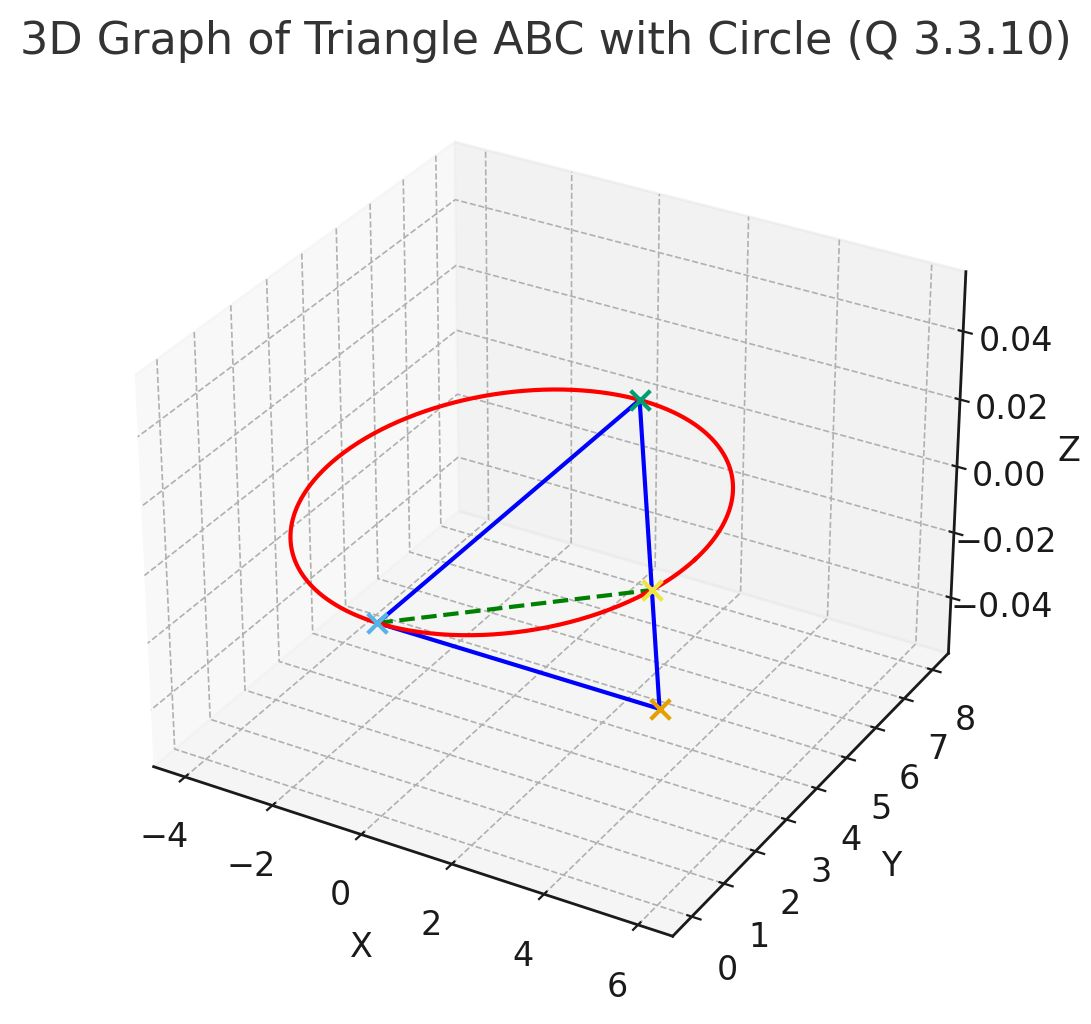
\includegraphics[width=0.5\linewidth]{beamer/figs/matg6.jpeg}
    \caption{}
    \label{fig:placeholder}
\end{figure}
\end{document}